\section{Absolute road coordinates}
\label{sec:roadcoord}

Because of limitations in hardware FPGA resources, calculating an (x,y) position with the ART hits in a road may be costly. To save resources, if we have small roads, i.e. 8-strip $X$,$U$,$V$ roads, we can assign an absolute (x,y) position to each unique set of $X$,$U$,$V$ roads. This is the position of the center of the diamond shown in Figure \ref{fig:cartoon_smallroads_1}. In the FPGA implementation, this would be reduced to a set of lookup tables. The performance of this is given in Figure \ref{fig:resolutions_cen}. This performs noticeably worse than using the ART strips in a road to calculate a position. The 3$\sigma$ y-residual RMS is 32.38 (33.45) $\pm$ 0.03 (0.03) mm for 0.5m (2.2m) long strips, which is about a factor of 3 worse than the calculation with strips. The 3$\sigma$ x-residual RMS is 0.07959 (0.7965) $\pm$ 0.0008 (0.0008) mm for 0.5m (2.2m) long strips. Using the strips, the x-residual RMS is 0.2969 (0.3019) $\pm$ 0.0003 (0.0003) mm for 0.5m (2.2m) long strips. However, with the added effect of $\delta$-rays, which we cannot simulate here, these two methods may be comparable.  

\begin{figure}[!htpb]
  \begin{center}
    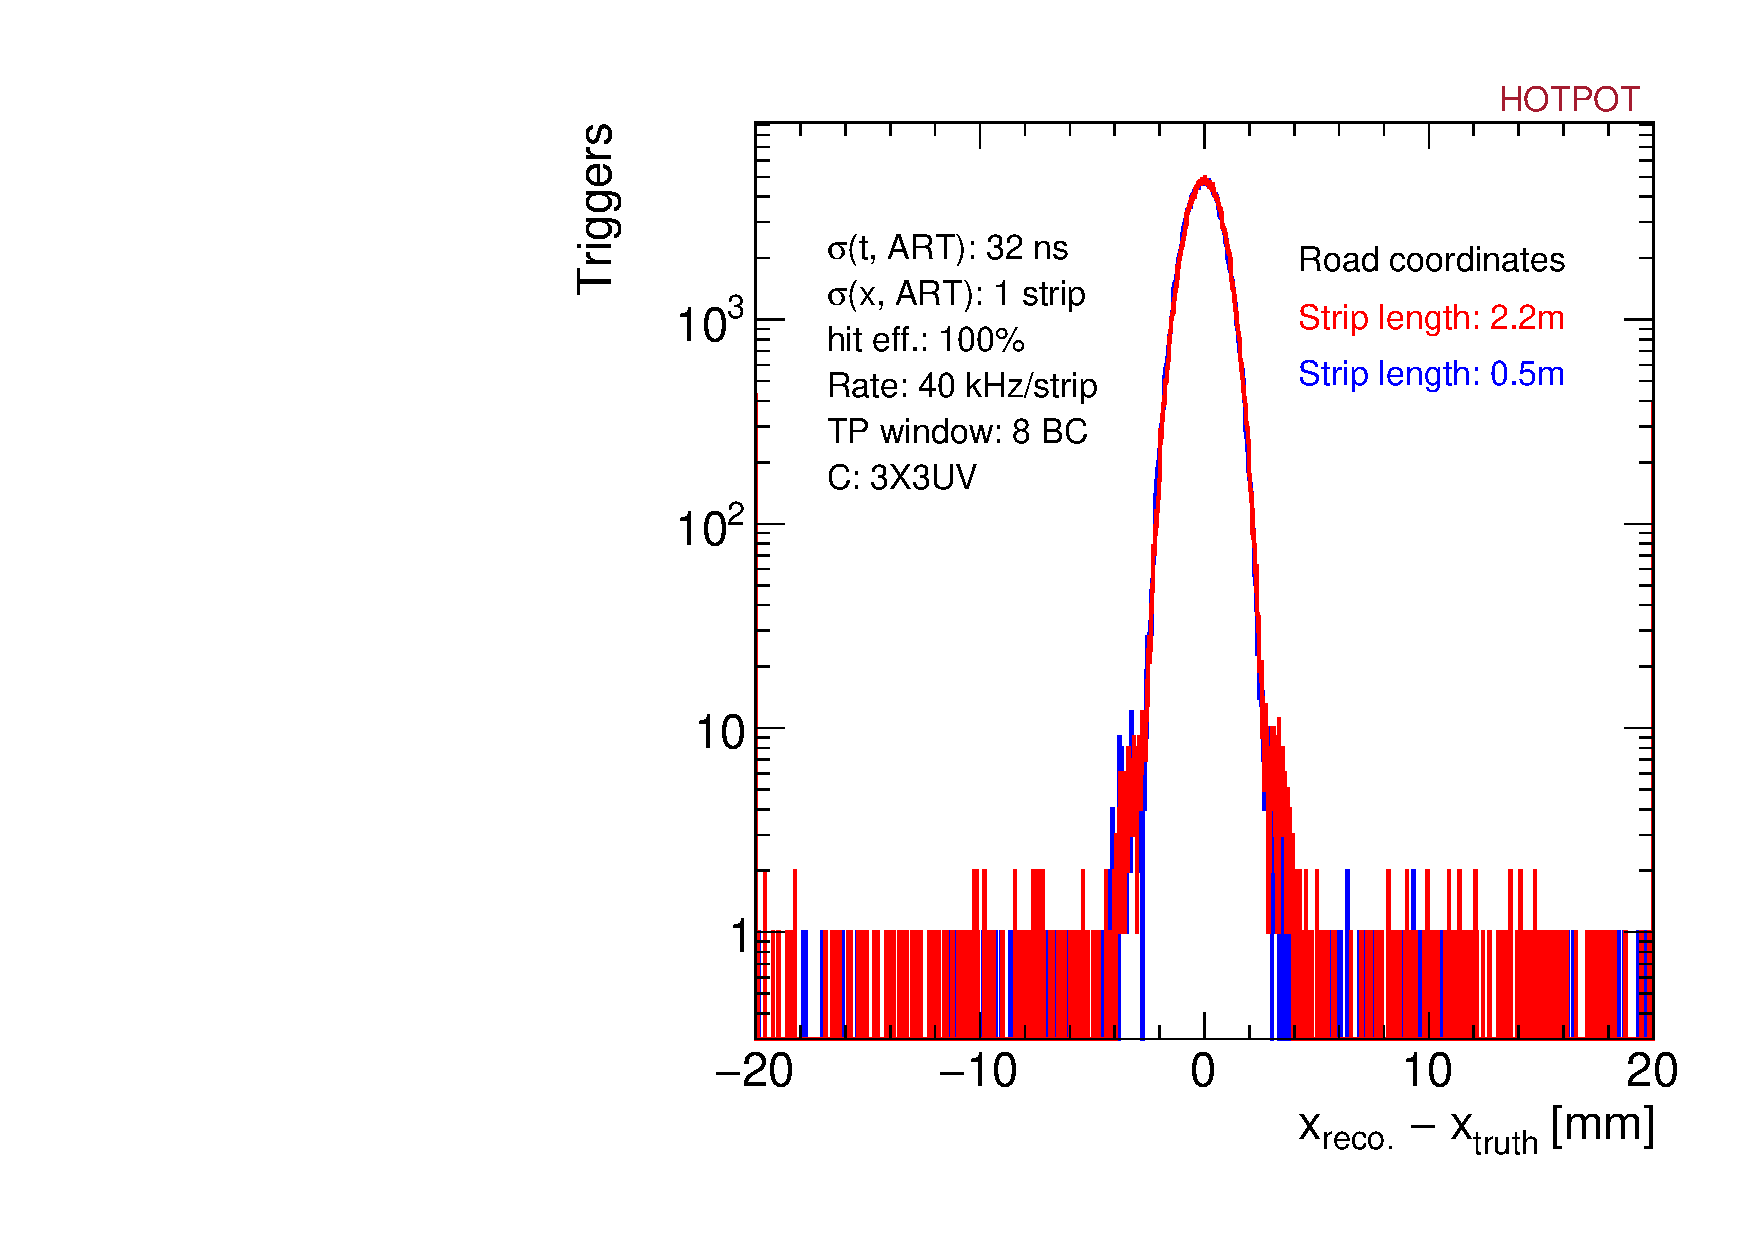
\includegraphics[width=0.48\textwidth]{figures/xres_cen.pdf}
    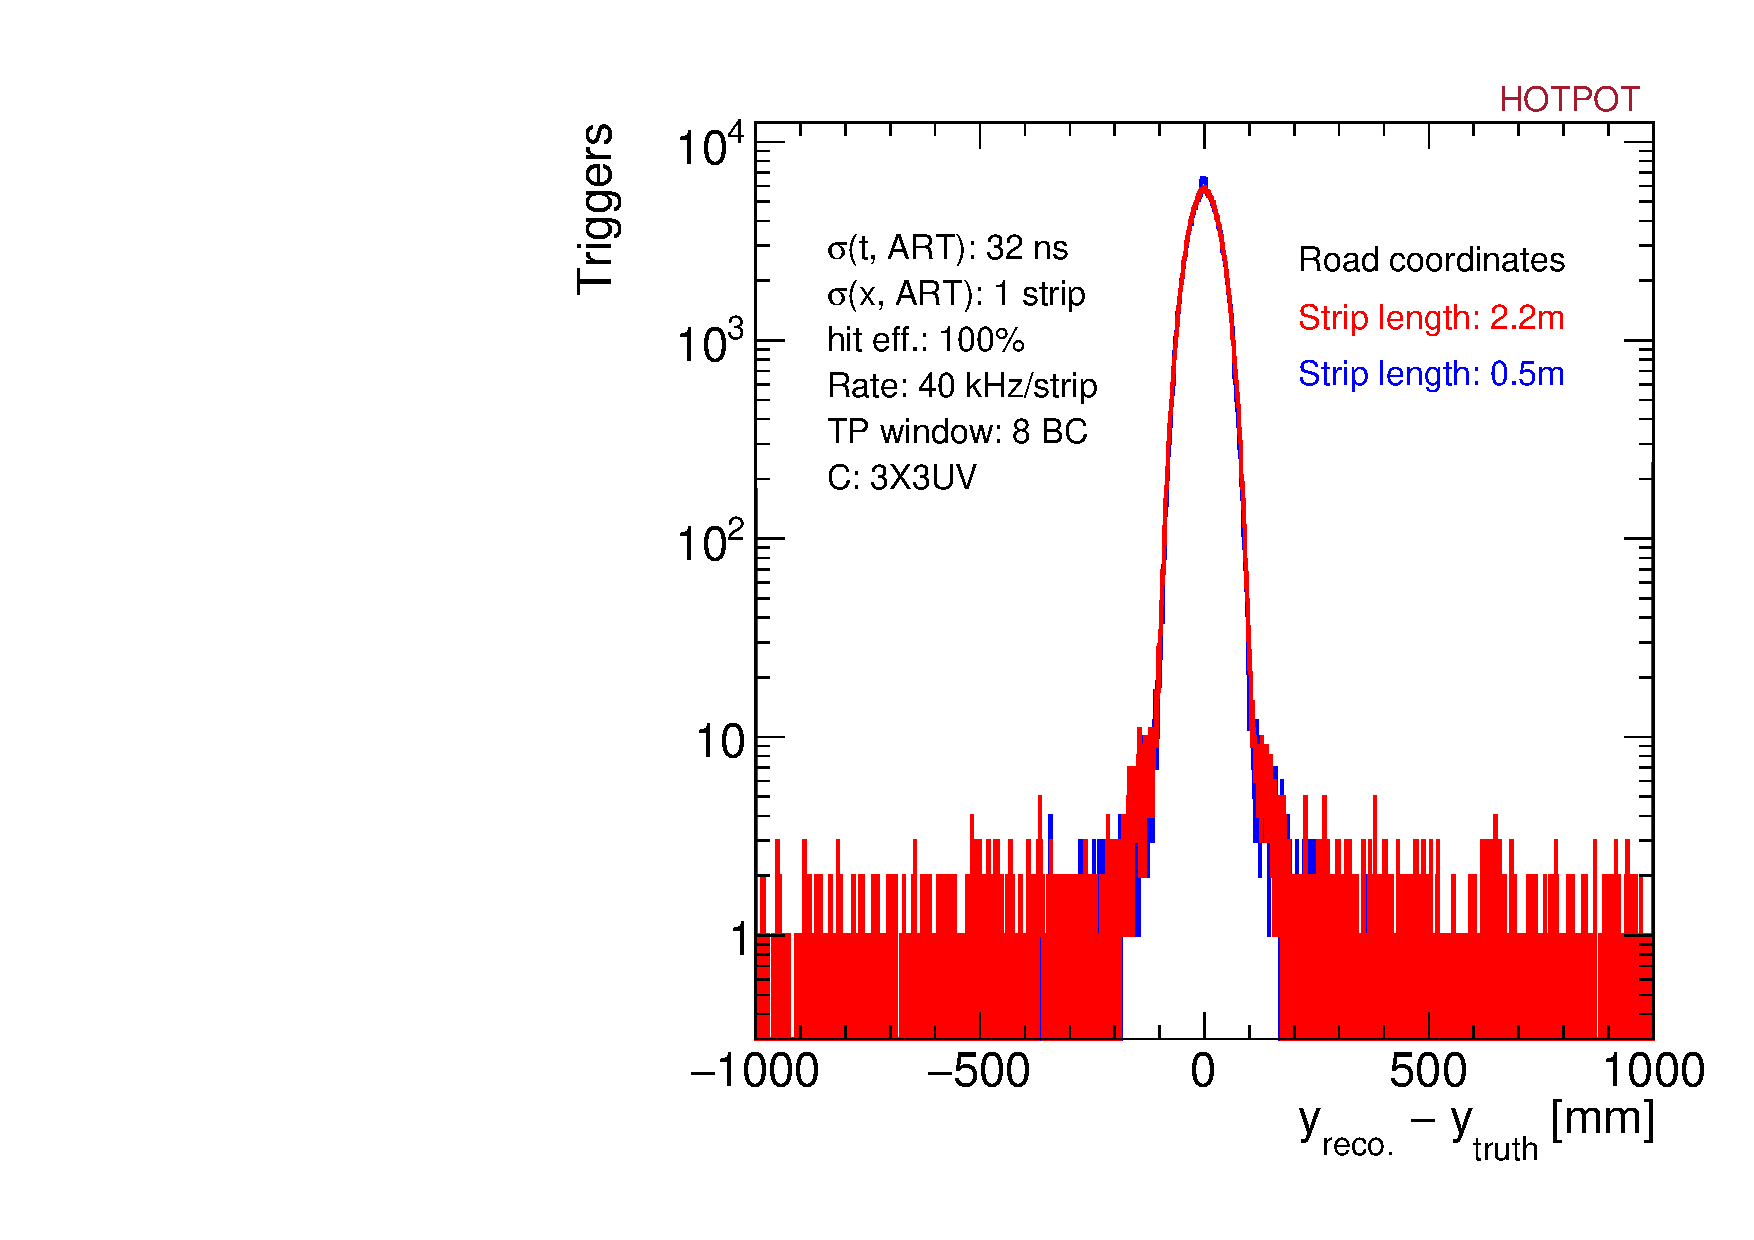
\includegraphics[width=0.48\textwidth]{figures/yres_cen.pdf}
  \end{center}
  \vspace{-10pt}
  \caption{Distribution of $x_\text{reco.} - x_\text{truth}$ (left) and $y_\text{reco.} - y_\text{truth}$ (right) for the proposed MMTP algorithm, where each unique set of $X$,$U$,$V$ roads is assigned a (x,y) position, with uncorrelated background at a rate of 40 kHz per strip.}
  \label{fig:resolutions_cen}
\end{figure}
